L'applicazione \emph{mobile} CAMUS rappresenta l'altro elemento fondamentale dell'ar\-chi\-tet\-tu\-ra. Fornisce all'utente finale l'interfaccia per accedere al sistema e semplifica l'utilizzo e l'accesso ai dati. Il capitolo si apre con una descrizione dettagliata delle \emph{Actions} e delle \emph{Stores} di \emph{Alt.js}.
%
Successivamente viene introdotto lo schema per definire le pagine e la logica di aggiornamento dei dati, seguendo il principio del flusso dati unidirezionale. In seguito viene definita la struttura del file di \emph{mashup} proveniente dal \emph{server}, che è indispensabile per la creazione delle schermate dell'app, per poi trattare nello specifico i metodi necessari per la costruzione di queste schermate.
Successivamente si illustra il flusso dei dati all'interno dell'applicazione e di come vengono gestite le richieste dati verso il \emph{server}, tramite GraphQL, per effettuare le attività riguardanti il \emph{login} e la ricerca delle informazioni contestuali per l'utente. In conclusione verrà trattato l'argomento riguardante i servizi di supporto.

\section{Gestione dello stato}\label{sec:state-management}
In questa sezione sono descritte nel dettaglio tutte le \emph{Actions} e le \emph{Stores} utilizzate nell'applicazione e presentate nella Sezione \ref{sec:action-store}

\subsection{Actions\label{sec:actions}}

Le \emph{Actions} sono i metodi utilizzati per modificare lo stato dell'ap\-pli\-ca\-zio\-ne. Vengono utilizzate principalmente in due modi:

\begin{itemize}
	\item \textbf{Data Fetching}
	Quando è necessario scaricare gli elementi necessari per il corretto funzionamento dell'applicazione (CDT e \emph{mashup}) o i dati provenienti dalle richieste, le \emph{action} hanno lo scopo di modificare lo stato per cambiare la \emph{view} dell'applicazione a seconda dello stato della richiesta.
	Per esempio, quando si preme il pulsante per effettuare una nuova richiesta basata sul contesto, viene invocata un'azione per mantenere lo stato coerente tra più componenti e permettere di mostrare in fase di caricamento uno \emph{Spinner}. Una volta che la richiesta viene evasa e i dati sono disponibili, viene eseguita un’altra azione per mostrarli all’interno di una \emph{ListView}
	\item \textbf{Application State}
	Lo stato generale dell'applicazione viene salvato utilizzando delle \emph{Action} chiamate dalle interazioni dell'utente con l'interfaccia grafica. Per esempio quando viene composto il contesto le diverse selezioni sono passate dall'utente tramite le \emph{Context Actions} nelle \emph{Context Store}, per poi rimanere disponibili per la visualizzazione delle selezioni già effettuate o la costruzione della \emph{query} per i dati
\end{itemize}	

Le \emph{Actions} implementate nell'applicazione sono le seguenti:

\begin{itemize}
	\item \textbf{User Actions}
	Sono le azioni che servono ad aggiornare i parametri relativi all'utente, come \emph{password}, \emph{email} e il suo identificativo della sessione:
	\begin{itemize}
		\item \textbf{Update Email}
		Metodo per aggiornare l'\emph{email} dell'utente 
		\item \textbf{Update Password}
		Metodo per aggiornare la \emph{password} dell'utente
		\item \textbf{Update Token}
		Metodo per tenere in memoria il \emph{token} della connessione col \emph{server}
	\end{itemize}
	\item \textbf{Context Actions}
	Sono le azioni che gestiscono la selezione del contesto, consentendo di modificare le scelte effettuate dall'utente:
	\begin{itemize}
		\item \textbf{Set Transport}
		Metodo per salvare la tipologia di trasporto da parte dell'utente
		\item \textbf{Set Typology}
		Metodo per salvare la tipologia nel caso di trasporto non con mezzi propri
		\item \textbf{Add Forbidden}
		Metodo per aggiungere un parametro in quelli da nascondere all'utente
		\item \textbf{Remove Forbidden}
		Metodo per rimuovere il parametro selezionato dalla lista di quelli da nascondere all'utente
		\item \textbf{Update Last Context}
		Metodo per salvare l'ultimo contesto inviato al \emph{server}, per poterlo riutilizzare nelle richieste per le pagine successive
	\end{itemize}
	\item \textbf{View Actions}
	Sono le azioni relative alla gestione dei \emph{mashup} ma non dello stato della navigazione, per le quali è utilizzato un componente aggiuntivo sempre basato su Flux (React Native Router Flux):
	\begin{itemize}
		\item \textbf{Set Views}
		Metodo per salvare il file con le \emph{view} provenienti dal \emph{server} 
		\item \textbf{Select Interest Topic}
		Metodo per salvare l'\emph{Interest Topic} selezionato dall'utente. Questa funzione è chiamata quando nella pagina iniziale l'utente seleziona l'\emph{Interest Topic} per la selezione della \emph{view} appropriata
	\end{itemize}
	
	\item \textbf{Data Actions}
	Trattano della gestione del CDT e dei risultati ottenuti dal \emph{server}:
	\begin{itemize}
		\item \textbf{Update Results}
		Metodo per aggiornare i dati dei risultati provenienti dalla \emph{query} basata sul contesto
		\item \textbf{Results Failed}
		Metodo per inviare il messaggio di errore proveniente dalla richiesta
		\item \textbf{Update Full CDT}
		Metodo per aggiornare il CDT associato all'utente
	\end{itemize}
\end{itemize}

\subsection{Stores\label{sec:stores}}

Le \emph{Stores} salvano lo stato dell'applicazione e forniscono alle \emph{view} nuovi dati ogni volta che sono aggiornate. 
Per ogni interazione sui dati dell'ap\-pli\-ca\-zio\-ne che necessitano di rimanere persistenti viene invocata una \emph{action} dal componente e dalla \emph{view} che si propaga prima nelle \emph{store} e successivamente aggiorna nuovamente la \emph{view}.
Si è scelto di suddividere le \emph{Store} per tipologia di operazione e dato trattata:

\begin{itemize}
	\item  \textbf{User Store}
	Nella \emph{User Store} sono memorizzati tutti i dati relativi all'utente. In particolare viene memorizzata la \emph{mail} dell'utente e l'identificativo del CDT a lui associato, che serviranno per poter effettuare le \emph{query} GraphQL per ottenere i dati
	\item \textbf{Context Store}
	Nel \emph{Context Store} vengono gestiti i dati che riguardano i dati di contesto, come le coordinate geografiche e le scelte delle tipologie di trasporto pubblico, in modo da essere riutilizzate. Per quanto riguarda le richieste di dati, una volta che il contesto viene composto per effettuare la prima \emph{query}, questo \emph{payload} viene salvato qui e poi riutilizzato nelle \emph{query} dei risultati successivi
	\item \textbf{View Store}
	In questa \emph{store} sono memorizzati tutti i dati relativi alle \emph{view}. Qui viene salvato lo schema di \emph{mashup} e l'\emph{Interest Topic} corrente
	\item \textbf{Data Store}
	Si tratta della \emph{store} più complessa perchè deve gestire in modo dinamico diverse tipologie di dato. Quando viene ricevuto il CDT vengono scanditi gli \emph{interest topic} è creato un oggetto nel campo \emph{results} che è composto da un \emph{array} di tanti oggetti definiti da due campi:
	\begin{enumerate}
		\item \textbf{Results}
		Rappresenta i risultati ricevuti per quell'\emph{interest topic}, comprende i dai servizi primari e i collegamenti per i servizi di supporto
		\item \textbf{Topic}
		Rappresenta l'\emph{Interest topic} associato ai risultati ricevuti dal \emph{server}
	\end{enumerate}
	Questa operazione è necessaria per poter gestire il fatto di avere comunque dei dati in memoria in condizioni di assenza di rete, anche per tipi diversi di risultati provenienti dal \emph{server} e per essere in grado di gestire una cardinalità variabile di tipologie di dati. Nel Listato \ref{lst:store-two-topics} è mostrato come viene rappresentato lo stato nel caso in cui l'utente abbia a disposizione due \emph{Interest Topic} e la suddivisione dei risultati per le due tipologie, in questo caso \emph{Restaurants} ed \emph{Event}. Si noti che oltre ai risultati sono salvati anche i parametri con lo stato della paginazione, per lasciare la possibilità di riprendere la visione di nuovi risultati.
\end{itemize}

\begin{listing}[H]
	\inputminted{json}{4-progettazione-alto-livello/Codice/store-two-topics.json}
	\caption{Esempio Data Store Mashup}
	\label{lst:store-two-topics}
\end{listing}

\section{Struttura dello schema di mashup\label{sec:struttura-schemi-mashup}}

Per poter permettere una dinamicità nella struttura delle schermate che formano l'applicazione si è scelto di utilizzare uno schema di \emph{mashup} molto semplice e allo stesso tempo in grado di fornire i parametri necessari all'applicazione per costruire le viste in tempo reale. Si è scelto di utilizzare una rappresentazione in JSON in modo da essere facilmente interpretabile all'interno del motore JavaScript di React Native. 
Nel caso di CAMUS sono considerate due tipologie di schema di \emph{mashup}: la \emph{list} e la \emph{details}. 
%cambiare questa frase 
Nella tipologia \emph{list} sono definite le \emph{view} che descrivono il singolo \emph{item} della \emph{ListView} e generalmente si compone di una quantità non eccessiva di componenti. 
Nel caso della \emph{list} sono definiti gli elementi da mostrare quando è presente la lista complessiva di risultati nella \emph{ListView}.
Nella tipologia \emph{details} sono disponibili tutti i dettagli dell'\emph{item} selezionato e sono definiti tutti i termini necessari a identificare l'elemento per l'utente.
Considerando l'esempio dei ristoranti, per la lista sono associati i termini che servono a identificare l'oggetto, come il nome e l'indirizzo. Se poi l'utente vuole vedere la mappa e visualizzare gli estremi per contattare il ristorante deve aprire la pagina dei dettagli, dove acquisendo i termini dal file di \emph{mashup}, sono visualizzati tutti i dettagli necessari per l'utente. Inoltre è specificata la tipologia dell'elemento da visualizzare, in modo da permettere all'\emph{app} di utilizzare le librerie di collegamento con le applicazioni specifiche del sistema operativo.

Nel Listato \ref{lst:mashup-schema} viene mostrato un esempio del file JSON di \emph{mashup} della pagina di dettaglio e in Figura \ref{fig:schermate-app-mashup} la sua traduzione nelle due versioni dell'applicazione.

\begin{listing}[H]
	\inputminted{json}{6-implementazione-app/Codice/mashup-schema-example-app.json}
	\caption{Esempio Schema Mashup}
	\label{lst:mashup-schema}
\end{listing}

\begin{figure}[ht]
	\begin{subfigure}{0.5\textwidth}
		\centering
		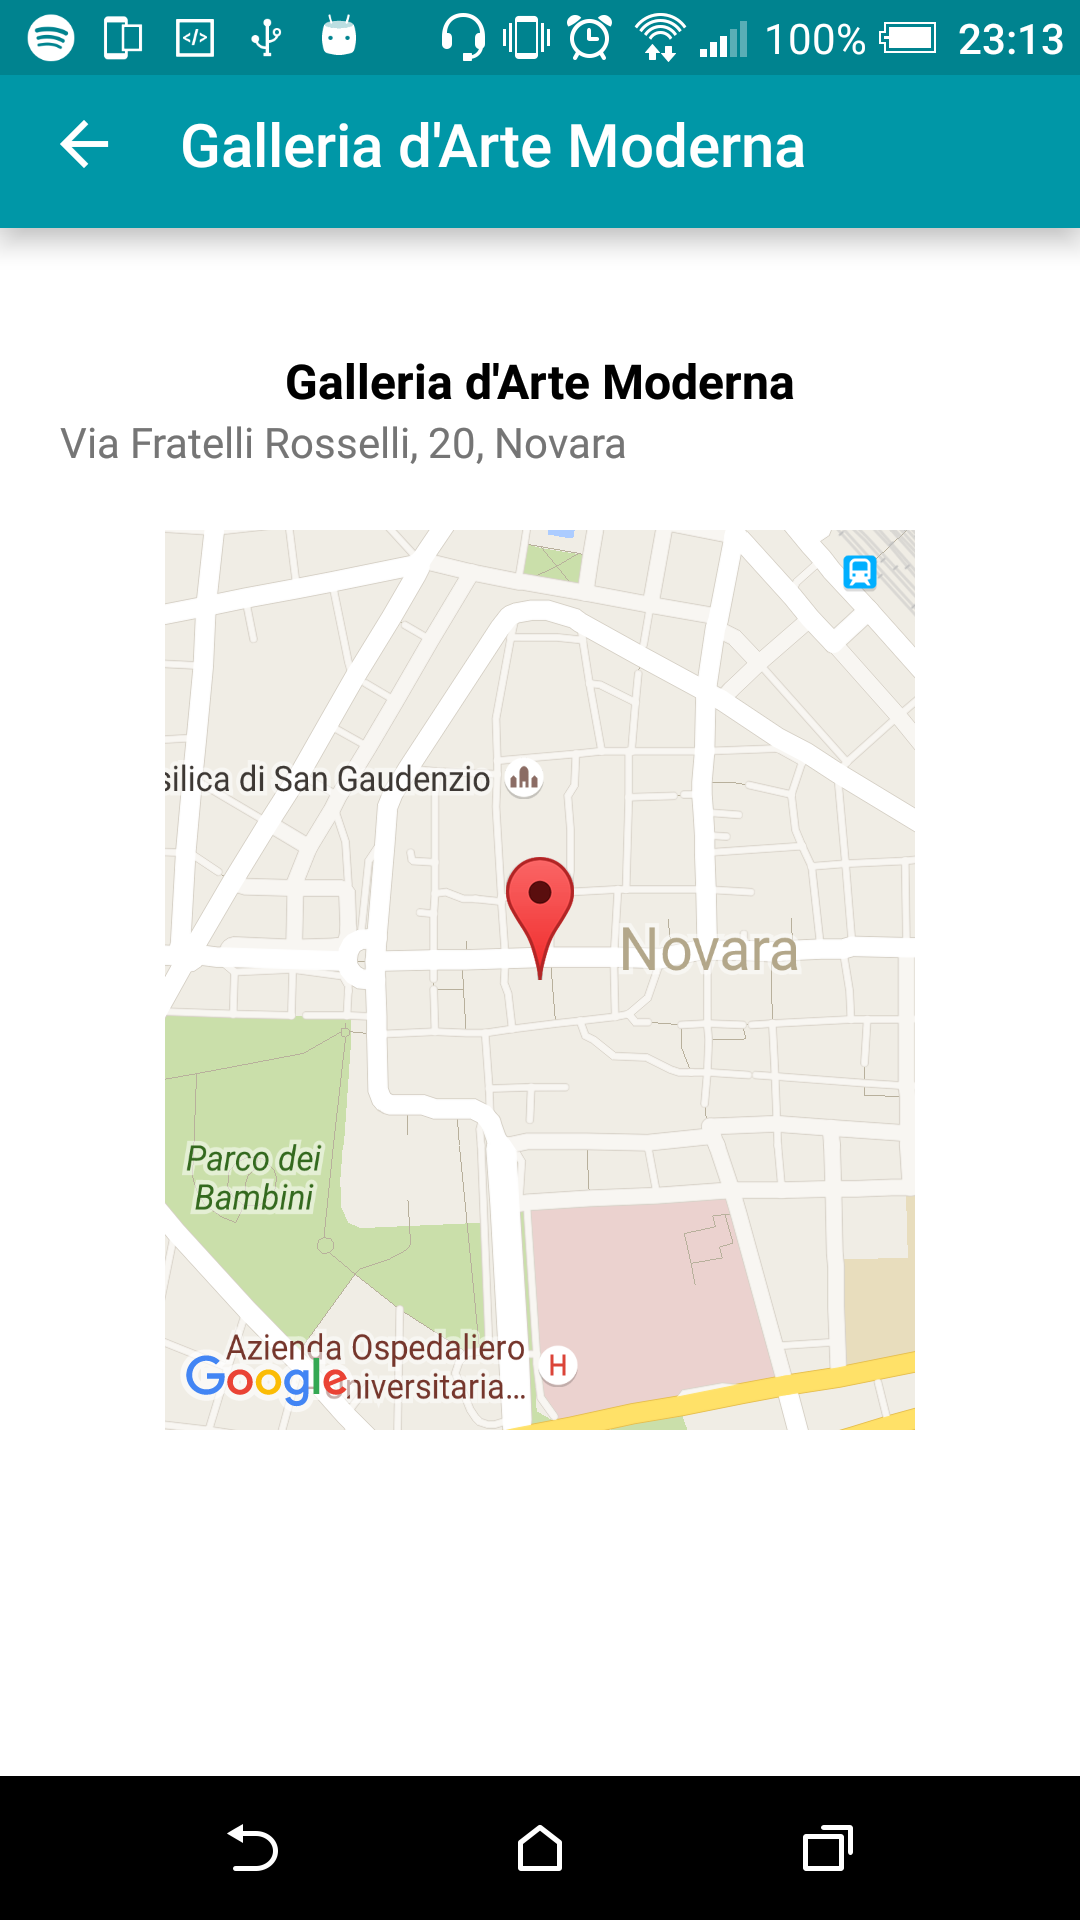
\includegraphics[width=0.48\textwidth]{6-implementazione-app/immagini/details_android.png}
		\caption{Versione Android}
	\end{subfigure}
	\begin{subfigure}{0.5\textwidth}
		\centering
		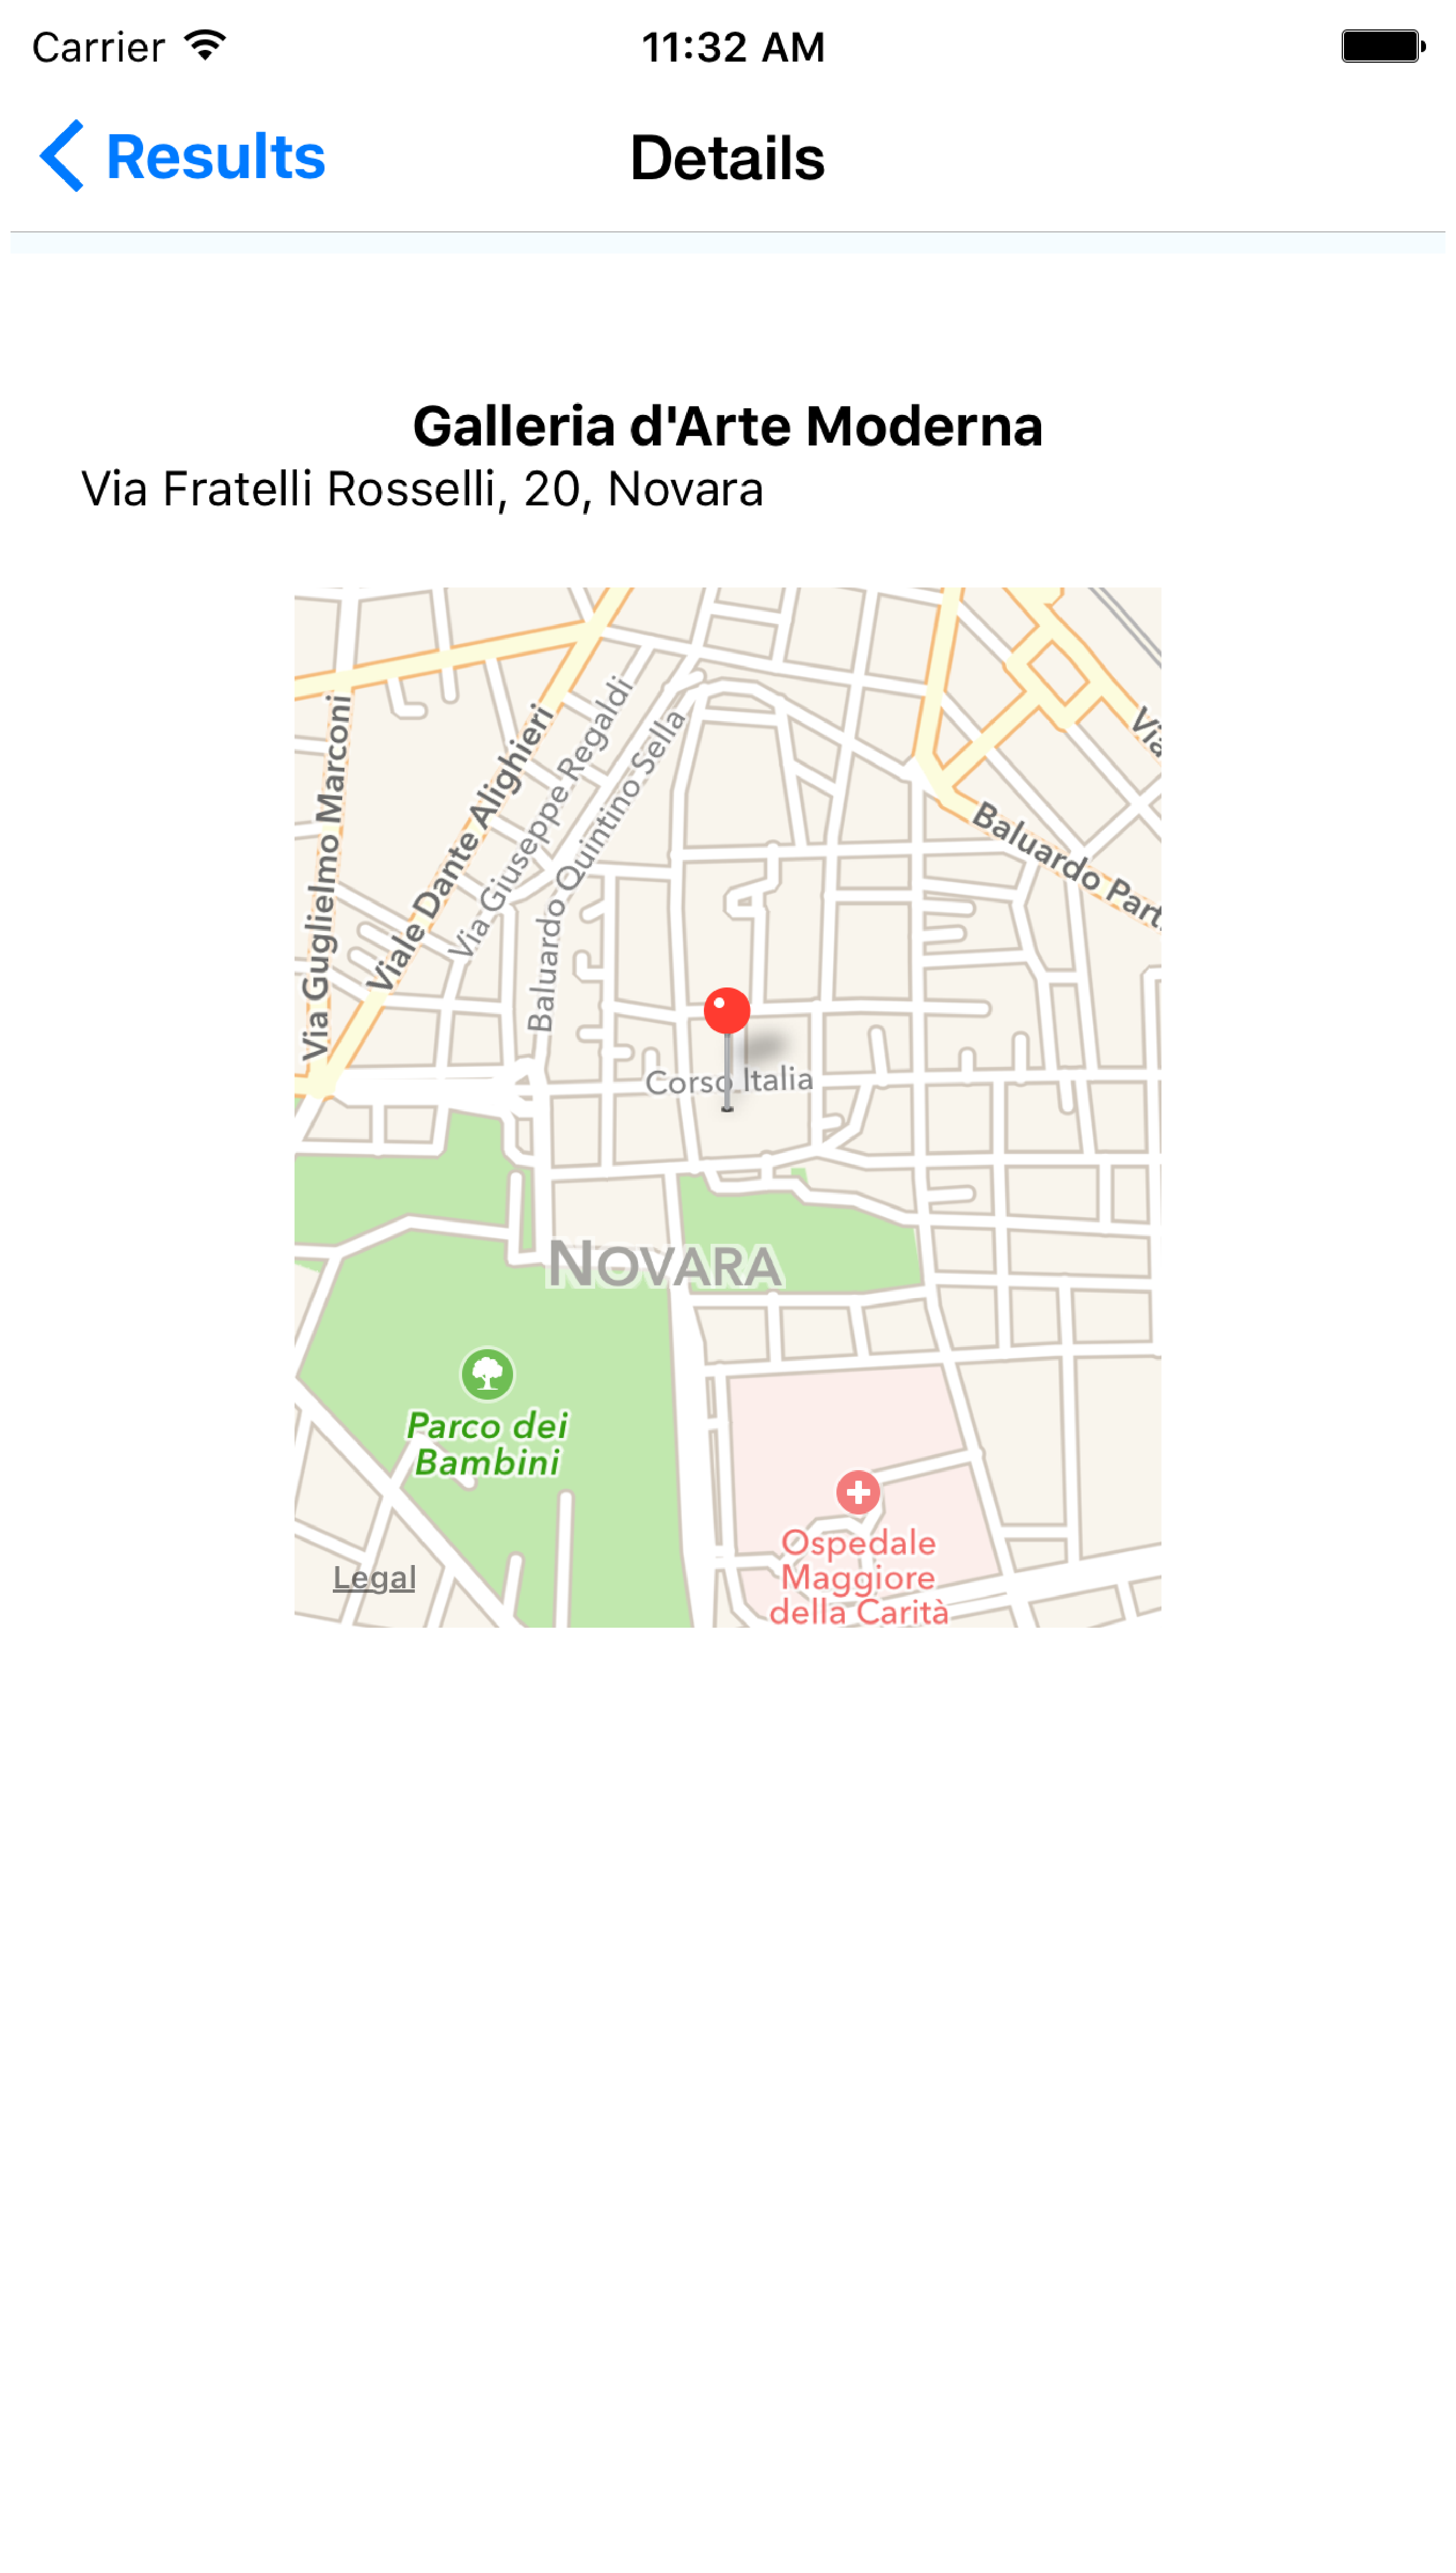
\includegraphics[width=0.48\textwidth]{6-implementazione-app/immagini/details_ios.pdf}
		\caption{Versione iOS}
	\end{subfigure}	
	\caption{Schermata dei dettagli}
	\label{fig:schermate-app-mashup}
\end{figure}

Di seguito sono elencate le diverse tipologie di dato che compongono l'oggetto che rappresenta i file di \emph{mashup}:

\begin{itemize}
	\item \textbf{Type}
	Il termine \emph{type} indica la tipologia dell'elemento da visualizzare nella \emph{view}. È associato a un componente React Native, che verrà richiamato nella fase di costruzione dell'interfaccia grafica
	\item \textbf{Topic}
	Si tratta di un \emph{array} di stringhe che indica tutte le aree di interesse associate allo schema in questione. Si è scelto di utilizzare una struttura basata su \emph{tag}: una volta che l’utente sceglie l’\emph{interest topic} viene utilizzato lo schema che lo possiede nei suoi \emph{tag} 
	\item \textbf{Contents}
	Indicano i termini del \emph{mashup} o dei nuovi componenti innestati. Se nell'oggetto padre è specificato un tipo gli elementi in \emph{contents} rappresentano i termini da richiedere nella \emph{query} GraphQL. In caso contrario questo campo indica che in \emph{contents} è presente un nuovo livello di annidamento. Ci possono essere tanti annidamenti, fino a quando non si arriva ad avere un oggetto che possiede il campo \emph{type}
	\item \textbf{Style}
	Questo campo serve per definire uno stile da assegnare al componente. Permette di personalizzare l’aspetto del componente, andando a ridefinire lo stile predefinito. Viene utilizzato Flexbox per la specifica degli stili
\end{itemize}

\section{Rendering delle view}\label{sec:rendering-view}

Si tratta della funzionalità più delicata da progettare all'interno dell'applicazione, perché non è così semplice pensare di generare in modo dinamico delle pagine con così tanta mutabilità a partire da un documento strutturato delle interfacce visuali.
Mentre in codice nativo questo problema può presentare delle difficoltà a livello implementativo, l'utilizzo da parte di React di un \emph{Virtual DOM} simile al linguaggio HTML offre il vantaggio di poter generare molto rapidamente una traduzione dal file di \emph{mashup} a un modello interpretabile dal motore di \emph{rendering} dell'\emph{app}.
Per questo motivo è stato creato un componente apposito, il \emph{View Builder}, che, dato un oggetto contenente lo schema di \emph{mashup}, riesce a gestire l'associazione dei contenuti semantici all'interno di questo schema con i componenti presenti nell'applicazione, restituendo il componente finale.
Sono presenti all'interno due tipologie di \emph{rendering}: il \emph{rendering} del contesto e il \emph{rendering} dei risultati.

\subsection{Rendering a partire dal contesto}

Il \emph{rendering} del contesto è basato esclusivamente su elementi provenienti dal CDT. Non si è reso necessario l'utilizzo di schemi di \textit{mashup}, in quanto tutti i dati occorrenti all'applicazione per costruire le \emph{view} sono già presenti all'interno del CDT. Per ogni elemento del CDT viene eseguita un'associazione a componenti già esistenti di \emph{React Native}, come per esempio \emph{Text} per mostrare il nome dell'elemento o \emph{Picker} in caso di selezioni multiple. Di seguito sono mostrati i diversi metodi di costruzione delle viste partendo dai singoli elementi del CDT:

\begin{itemize}
	\item \textbf{Interest Topic}
	Gli \emph{Interest Topic} hanno bisogno di essere selezionati nella pagina iniziale una volta effettuata l'autenticazione e caricati in una lista di pulsanti con due elementi per riga e con un'icona rappresentativa. I pulsanti e le icone sono predefinite nell'applicazione e necessitano soltanto di una associazione <\emph{nome},\emph{elemento}> dal campo \emph{Interest Topic} del CDT. Questa funzione molto semplice viene eseguita direttamente all'interno della pagina principale senza la necessità di utilizzare il \emph{View Builder}
	\item \textbf{Altri elementi}
	Gli altri elementi del contesto sono elaborati all'interno del componente \emph{View Builder}. Con una funzione ricorsiva viene scandito l'intero CDT ricevuto dal \emph{server} con i campi da modificare e in base ai contenuti viene costruito l'elemento della \emph{view}, a seconda della tipologia. Per esempio, se per un campo è richiesto l'inserimento di un numero verrà mostrato un \emph{TextInput} che permette il completamento solo con numeri, mentre se è necessario effettuare una scelta tra più elementi verrà mostrata una lista selezionabile.
	Assume una grande importanza anche la gestione delle esclusioni tra le operazioni. Se viene selezionato \virgolette{With Car} non è corretto mostrare le possibili tipologie di trasporto pubblico, perché si conosce già a priori che l'utente non selezionerà mai nello stesso momento come mezzo di trasporto l'automobile e il bus. Per questo scopo viene utilizzato il parametro \emph{parents} presente in ogni elemento del CDT; se il valore è stato selezionato dall'utente, allora gli sono mostrate tutte le sottocategorie. Per esempio quando l'utente seleziona \virgolette{With Car} non gli sono proposte tipologie diverse di trasporto con l'auto, mentre se seleziona \virgolette{Public Transport} allora può scegliere una categoria ben definita di trasporto pubblico, a seconda delle sue esigenze
\end{itemize}
	
\subsection{Rendering dei risultati}\label{sec:view-risultati}

Per quanto concerne i risultati ottenuti dalle \emph{query} GraphQL elaborate dal server, entrano in gioco in maniera preponderante gli schemi di \emph{mashup}. Per i motivi spiegati nella Sezione \ref{sec:mashup-design}, la risoluzione del problema necessita di un funzionamento più complesso rispetto alla visualizzazione del contesto. La funzione di \emph{rendering} per quanto riguarda i risultati è la medesima sia per la lista che per i dettagli, quello che cambia è il contenitore del componente \emph{View Builder}: per la lista è un figlio nel metodo di \emph{renderItem()} della \emph{ListView}, mentre per i dettagli definisce l'intera pagina.
Al componente \emph{View Render} sono necessari due oggetti: il file di \emph{mashup} e i dati del singolo risultato.
Si suppone che nel file di \textit{mashup} gli elementi siano già stati generati in ordine di visualizzazione, perché nella funzione di costruzione delle \emph{view} non è possibile modificare tale ordine. Tuttavia è possibile modificare lo stile più esterno del componente risultante per cambiare il \emph{layout} dei figli del \emph{View Builder}. Per prima cosa il \emph{View Builder} deve scegliere le \emph{view} associate all'\emph{Interest Topic} facendo una ricerca della prima vista che contiene il valore corrente dell'\emph{Interest Topic} e passare questo oggetto alla funzione di \textit{rendering}. A questo punto si è pronti per costruire la \emph{view} del componente: viene scandito ogni elemento del file di \textit{mashup} e si associa il valore dato dal termine dell'oggetto del risultato e viene restituito il componente pronto per essere elaborato per la visualizzazione. Nel caso in cui non fosse presente un valore per il termine desiderato ovviamente non viene visualizzato alcun elemento, si restituisce una \emph{view} base vuota, che non ha nessuna incidenza sulla grafica avendo dimensione nulla. Nel caso in cui esista un oggetto di tipo \emph{style}, esso ha la priorità rispetto a quello presente nel foglio di stile predefinito dell'applicazione. Nel prototipo sono disponibili queste tipologie di componenti specificabili nel campo \emph{type} dell'oggetto di \textit{mashup}:

\begin{itemize}
	\item \textbf{Text}
	\upe il componente utilizzato per mostrare informazioni testuali. Per la sua personalizzazione si utilizzano attributi diversi nel foglio di stile in comune per tutta l'applicazione o le specifiche presenti nell'attributo \emph{style} del \textit{mashup}
	\item \textbf{Map}
	\upe il componente che visualizza le mappe. Presenta due implementazioni differenti per quanto riguarda iOS e Android, poiché come mappe di sistema utilizzano due applicazioni differenti. iOS mette a disposizione le mappe di Apple, già integrate nel componente \emph{MapView} fornito da React Native, mentre per Android vengono utilizzate le mappe di Google Maps, per le quali è stato utilizzato un modulo aggiuntivo
	\item \textbf{Website}
	Viene utilizzato per gli indirizzi web. Permette di aprire il collegamento direttamente nel \emph{browser} del dispositivo
	\item \textbf{Email}
	Permette di visualizzare l'indirizzo \emph{mail} associato all'elemento, selezionando l'icona di invio \emph{email} l'utente viene reindirizzato all'applicazione o alla scelta di un'applicazione per comporre un messaggio da inviare all'indirizzo specificato
	\item \textbf{Phone}
	Questo componente gestisce il numero di telefono dell'elemento, con la possibilità di inviare un messaggio al numero specifico o di effettuare una telefonata, sempre utilizzando le applicazioni predefinite del dispositivo mobile
	\item \textbf{Support}
	Si tratta del componente che gestisce i servizi di supporto con i collegamenti alle applicazioni esterne, verrà spiegato nel dettaglio nella Sezione \ref{sec:servizi-supporto-app}
\end{itemize}

\subsection{Gestione degli stili}

Per quanto riguarda la gestione degli stili si è scelto di adottare una soluzione molto semplice, ma allo stesso tempo molto efficace. Si è partiti dalla condizione che React Native utilizza come gestione dello stile Flexbox\footnote{Flexbox su W3Schools: \url{Htp://www.w3schools.com/css/css3_flexbox.asp}}, che è una variante basata sugli stili CSS ottimizzata per la gestione degli elementi che necessitano di adattarsi a differenti dimensioni degli schermi. Il linguaggio utilizzato risulta essere molto simile a JSON e quindi è facilmente integrabile in JavaScript. L'elemento che gestisce gli attributi grafici è lo \emph{StyleSheet}, che espone l'oggetto \emph{styles} e gli attributi \emph{PRIMARY\_COLOR} e \emph{SECODARY\_COLOR}.
Nell'oggetto \emph{styles} sono impostati tutti gli stili di ogni componente grafico dell'applicazione che vengono richiamati nella fase di costruzione delle \emph{view}. In questo modo ogni modifica all'interno dell'oggetto si ripercuote in tutta l'applicazione.
I due attributi per la gestione dei colori sono risultati indispensabili in particolare per alcuni componenti, come la \emph{StatusBar} di Android, che hanno come elemento impostabile solo il colore e non lo stile completo. Ovviamente la modifica all'interno dello \emph{StyleSheet} dei parametri di colore è necessaria solo in un punto del codice, in modo da propagarsi in modo coerente per l'intera applicazione.
Nel Listato \ref{lst:stylesheet} viene mostrato un esempio del foglio di stile utilizzato nell'applicazione. Si noti come i parametri che definiscono ogni singolo elemento sono abbastanza autoesplicativi, fornendo allo sviluppatore una maggiore semplicità di programmazione. Diversi parametri sono stati ripetuti, per permettere la visualizzazione del componente in modo ottimale sia in Android che in iOS.

\begin{listing}[H]
	\inputminted{js}{6-implementazione-app/Codice/stylesheet.js}
	\caption{Esempio Foglio di Stile}
	\label{lst:stylesheet}
\end{listing}

\section{Query GraphQL}\label{sec:utilizzo-dati-app}

In questa sezione si vuole affrontare la gestione dei dati all'interno dell'applicazione, partendo dagli algoritmi per costruire le \emph{query} GraphQL per poi parlare della gestione della paginazione.
Tutto lo scambio di dati tra l'applicazione e il \emph{server} viene svolto utilizzando \emph{query} GraphQL, come spiegato nella Sezione \ref{sec:architettura-backend}. Per implementare il modulo di gestione delle connessioni si è scelto di utilizzare \emph{Lokka}\footnote{Lokka: \url{https://github.com/kadirahq/lokka}}, un \emph{client} compatibile con GraphQL che permette di gestire le \emph{query} come se fossero normali \emph{fetch()} di JavaScript e lasciare una configurazione più libera e adattabile alle esigenze del sistema. Questo si sposa bene con il paradigma Flux, in quanto permette il salvataggio della maggior parte del contenuto della risposta nella \emph{Data Store} con le modalità esposte nella Sezione \ref{sec:action-store} e rendendolo quindi disponibile per tutti i componenti dell'applicazione. Di seguito sono spiegate le due tipologie principali di \emph{query} gestite con GraphQL, ossia le \emph{query} di login e le \emph{query} per accedere ai dati.

\subsection{Login Query}

Le \emph{query} per gestire il meccanismo di \emph{login} sono molto semplici. Sono basate sui dati inseriti dall'utente quando si trova nella \emph{Login Page} e sulle risposte intermedie fornite dal \emph{server}. Queste \emph{query} servono per ottenere l'identificativo del CDT associato all'utente e lo schema dei \emph{mashup} con le definizioni delle sue \emph{view}.
I dati necessari per la costruzione della \emph{query} sono l'indirizzo \emph{email} e la \emph{password}, che sono inseriti dall'utente nella prima pagina che gli viene mostrata. Questi dati vengono salvati nella \emph{User Store} e sono conservati nello stato dell'applicazione, nel caso in cui fosse necessario effettuare una nuova richiesta. Nel caso in cui l'indirizzo \emph{email} e/o la \emph{password} siano errati viene notificato un errore mentre se uno dei due campi è mancante vengono richiesti nuovamente senza inviare nessuna richiesta.
In caso di risposta affermativa viene restituito all'utente un \emph{token}, generato ogni volta che l'utente effettua l'autenticazione. Questo \emph{token} viene salvato sempre nella \emph{User Store} e successivamente inviato al \emph{server} con la \emph{query} \emph{getPersonalData()} per ottenere il CDT e lo schema di \emph{mashup} associati all'utente.

\subsection{Data Query} \label{sec:data-query}

Le \emph{query} per gestire i dati necessitano di tutta una serie di operazioni preliminari perché sono presenti diversi parametri da ricavare per poter formare una richiesta GraphQL. Oltre alla definizione spiegata nella Sezione \ref{sec:endpoint-graphql}, di seguito viene spiegata la modalità di costruzione dei parametri che sono necessari per la composizione della query utilizzando il metodo \emph{client.query()} di \emph{Lokka}:

\begin{itemize}
	\item \textbf{Email}
	Si tratta della \emph{mail} inserita dell'utente
	\item \textbf{IdCdt}
	Rappresenta l'identificativo del CDT, il quale appartiene a ogni singolo utente
	\item \textbf{Context}
	\upe l'oggetto che rappresenta il contesto attuale nel quale si trova l'utente. Quando l'utente ha terminato la compilazione del contesto nella \emph{Context Selection Page} i parametri e i valori sono registrati nella \emph{Context Store} ma, per essere interpretati dal \emph{server}, necessitano di una conversione in un oggetto ben definito. Il problema di una \emph{query} GraphQL è che l'oggetto in questione deve essere ulteriormente convertito in una stringa unica per poi venire collocato come \textit{payload} nella POST/HTTP. Per svolgere questo compito viene utilizzata una funzione personalizzata che permette di mantenere inalterata la chiave degli oggetti JavaScript e produce in uscita una stringa. Per poter convertire anche gli oggetti che sono innestati a un livello superiore viene utilizzata una ricorsione che richiama la prima funzione. \upe necessario risolvere anche un altro problema, cioè quello legato ai valori del CDT che possiedono il parametro \virgolette{Parents}. In questo caso non è corretto inviare entrambi i parametri, ma solamente quello figlio: è poi il server che ha la capacità di comprendere che è selezionato anche il parametro padre. Per esempio se si considera il parametro \virgolette{Public Transport}, si hanno due possibilità. La prima è che se l'utente non seleziona alcuna categoria allora l'applicazione invia l'oggetto così com'è nella \textit{query}, ma viene chiamato la \emph{Action} delle \emph{ContextActions} \virgolette{removeForbidden()} che, nel caso in cui sia stata selezionata in precedenza una tipologia che aveva come padre \virgolette{Public Transport}  . La seconda è che l'utente selezioni una tipologia specifica, come \virgolette{Bus}: l'applicazione chiama la \emph{Action} \virgolette{addForbidden()} e il valore \virgolette{Public Transport} viene inserito nell'elenco degli elementi da non considerare mentre viene costruita la \textit{query}
	\item \textbf{Support}
	Rappresenta la tipologia di servizi di supporto che l'utente richiede per integrare al meglio i dati che gli necessitano %Per esempio nella demo di CAMUS si utilizzano i servizi di tipo \virgolette{Transport}
	\item \textbf{PrimaryResults}
	Rappresenta lo schema dei dati che devono essere restituiti dai servizi invocati dal \emph{server} per costruire l'insieme dei risultati per l'utente. GraphQL permette di eseguire delle richieste di dati altamente personalizzate, permettendo di richiedere la minima quantità di dati indispensabili per l'utilizzo da parte dell'utente. Per poter svolgere questo compito si è scelto di utilizzare i termini semantici dei \emph{mashup}, in particolare della tipologia \emph{details}, perché si suppone che nel caso della lista si abbia un sottoinsieme dei termini semantici. Come per la funzione di costruzione della \emph{view} espressa nella Sezione \ref{sec:rendering-view}, anche in questo caso è necessario acquisire lo schema associato all'\emph{Interest Topic} e poi selezionare i termini, per creare l'oggetto GraphQL che definisce i \emph{Primary Results}. Considerando l'esempio di schema del Listato \ref{lst:mashup-schema} si può notare come i termini nel campo \emph{contents} siano \virgolette{title}, \virgolette{address}, \virgolette{longitude}, \virgolette{latitude} e \virgolette{meta}. Come oggetto GraphQL è necessario passare tutti questi termini all'interno di \emph{Primary Results} in un formato dove l'unico separatore è il carattere \virgolette{a capo}, per ottenere un risultato simile a quello nella Figura \ref{lst:esempio-query-graphql} 
	\item \textbf{SupportResults}
	Lo stesso meccanismo utilizzato per i \emph{PrimaryResults} viene riproposto anche per i risultati di supporto. Invece di recuperare i \emph{mashup} dalle \emph{Store} viene riproposta la stessa definizione per ogni \emph{query}, perché i servizi di supporto sono definiti sempre nello stesso modo con i campi \emph{category}, \emph{service}, \emph{url} e \emph{storeLink}
\end{itemize}

\subsection{Gestione paginazione}\label{sec:paginazione-app}

Per quanto riguarda la gestione dei risultati l'applicazione sfrutta la paginazione messa a disposizione da GraphQL. A livello \emph{client} viene implementata quando viene restituito il risultato della \emph{query} basata sul contesto, per velocizzare e ottimizzare lo scambio dati col \emph{server}. Nel modulo \emph{Connection Manager} sono implementati due metodi diversi per creare le \emph{query}, uno per la prima richiesta e un altro per le successive. Si tratta di due richieste non molto differenti tra loro:

\begin{enumerate}
	\item \textbf{Richiesta iniziale}
	Nella richiesta iniziale è necessario acquisire i parametri del contesto costruiti dalle \emph{Context Selection Page} e gli oggetti ricavati dai parametri definiti dall'utente e dai sensori, sotto forma in stringhe. Inoltre vengono definiti i parametri sulle dimensioni della pagina, ma senza nessun riferimento agli elementi precedenti.
	I parametri dell'oggetto ritornato dal \emph{server} che contiene le informazioni necessarie all'applicazione per richiedere le pagine successive è specificato nella Sezione \ref{sec:execute-query-endpoint}
	\item \textbf{Richiesta pagine successive}
	Quando vengono richieste le pagine successive è sbagliato far ricavare nuovamente dai sensori e dall'utente il contesto, perché non è detto che questo rimanga statico. Per esempio se l'utente è in viaggio in treno le coordinate geografiche cambiano molto velocemente e quindi per il \emph{server} si tratta di un nuovo contesto, che implica la restituzione di un nuovo insieme di risultati. In questo modo si potrebbero ottenere dal \emph{server} dei dati diversi. Per risolvere questo problema si è scelto di memorizzare nella \emph{Context Store} i parametri immutabili della prima richiesta, come quelli di contesto, le definizioni dei dati e i servizi di supporto. La nuova \emph{query} quindi recupera l'identificativo dell'ultimo elemento restituito dalla \emph{query} della pagina precedente, ponendo quest'ultimo come parametro \emph{after} e mantenendo costante la dimensione della pagina
\end{enumerate} 

Questi due metodi sono chiamati dall'applicazione in due fasi differenti: la richiesta iniziale viene invocata quando l'utente ha appena definito il contesto e richiede nuovi dati, la richiesta delle pagine successive quando l'utente si trova nella \emph{Results Page} e scorre fino in fondo la lista di risultati. 
Il \emph{server} riesce a gestire lo stato delle richieste come spiegato nella Sezione \ref{sec:descrittore-paginazione} e l'applicazione deve stare attenta solamente a controllare il campo che indica l'esistenza o meno di una pagina successiva.
Considerando sempre il Listato \ref{lst:esempio-risposta-data-app}, viene mostrata una risposta a una \emph{query} iniziale con numero di risultati nel parametro \emph{first} impostato a \emph{5}, e con il parametro \emph{hasNextPage} uguale a \emph{true} per indicare che esistono ulteriori pagine da acquisire. Nel caso in cui l'utente voglia visualizzare altri risultati è necessario eseguire una richiesta di una nuova pagina. Nella \emph{query} per la seconda pagina è necessario aggiungere il parametro \emph{after} seguito dall'identificativo dell'ultimo elemento della risposta precedente assieme al parametro \emph{first} con lo stesso valore della richiesta precedente. A questo punto, essendoci già presenti dei risultati nella \emph{Data Store}, i nuovi risultati vengono concatenati assieme a quelli esistenti e aggiornano la \emph{view} posizionandoli in coda a quelli già mostrati. Come ulteriore ottimizzazione nell'implementazione della \emph{ListView} è possibile impostare un'azione nel recuperare delle \emph{view} quando si giunge a una certa distanza prestabilita dalla fine della pagina. Quindi la richiesta della pagina successiva viene eseguita poco prima di raggiungere il termine della lista, fornendo all'utente un'esperienza d'uso migliore.

\section{Servizi di supporto}\label{sec:servizi-supporto-app}

I servizi di supporto sono utilizzati esclusivamente nell'applicazione. Quando viene effettuata una richiesta viene inserita la tipologia desiderata di servizi di supporto e il \emph{server} restituisce un indirizzo che l'applicazione può gestire in diversi modi:

\begin{itemize}
	\item \textbf{Web Linking}
	L'applicazione riceve un \emph{link} per accedere all'\emph{endpoint} del servizio, richiede i dati e li visualizza all'interno del componente preposto dell'\emph{app}. Questa soluzione è gestita mediante una funzione del \emph{Connection Manager} che gestisce le \emph{query} nella modalità richiesta dal servizio da interrogare
	\item \textbf{Deep Linking}
	I \emph{Deep Link} sono degli URI che permettono di lanciare una applicazione preinstallata sul dispositivo. Sono collegamenti molto simili agli URL HTTP, con la differenza che viene specificato il nome che identifica l'applicazione da lanciare. Se l'applicazione desiderata non è presente sul dispositivo è necessario gestire l'errore e reindirizzare l'utente sull'App Store o sul Google Play Store per poterla scaricare. Questa tipologia di collegamenti migliora l'integrazione dell'applicazione CAMUS con l'intero sistema operativo
\end{itemize}
	 
In generale il funzionamento di queste tipologie di collegamenti è gestito dall'ap\-pli\-ca\-zio\-ne con le stesse modalità. Nel risultato proveniente dal \emph{server} viene restituito un \emph{link} del tipo \emph{nomeapp://?param={value}} e l'applicazione è in grado di sostituire al posto di \emph{value} il valore proveniente dall'elemento dei risultati per poter aprire l'applicazione di supporto. La scelta che è stata fatta è di utilizzare due \emph{link} diversi per ogni sistema operativo: il primo punta all'applicazione installata sul dispositivo, mentre il secondo allo \emph{store} predefinito per scaricare l'applicazione. Questa scelta permette di definire applicazioni diverse o di usare la stessa applicazione nel caso in cui utilizzi \emph{link} diversi a seconda del sistema operativo. Un esempio di applicazione che ha questo problema è Google Maps: in Android l'URI è del tipo \emph{google.navigation:q={value}}, mentre in iOS è del tipo \emph{comgooglemaps://?saddr={value}}. In React Native la libreria di \emph{Linking} è in comune tra le diverse piattaforme e quindi è necessario prestare attenzione al collegamento che viene passato. Nell'applicazione questo viene implementato con il metodo \emph{Linking.canOpenUrl(URI)} nel quale viene passato al suo interno il \emph{link} da aprire. Se il metodo ritorna un errore allora viene aperto il collegamento che punta allo \emph{store} mentre in caso di risposta affermativa l'applicazione desiderata viene aperta. Nel Listato \ref{lst:esempio-support-app} viene rappresentato un esempio completo dell'oggetto che rappresenta il servizio di supporto proveniente dal \emph{server}, dove:

\begin{itemize}
	\item \textbf{Category}
	Indica la categoria di appartenenza del servizio
	\item \textbf{Service}
	Rappresenta il nome del servizio
	\item \textbf{Url}
	Indica l'URL per invocare il servizio o aprire l'applicazione
	\item \textbf{Store Link}
	Rappresenta il \emph{link} nello \emph{store} di sistema per scaricare l'ap\-pli\-ca\-zio\-ne se non è installata sul dispositivo  
\end{itemize}

\begin{listing}[H]
	\inputminted{json}{6-implementazione-app/Codice/esempio_supporto_app.json}
	\caption{Esempio di servizi di supporto con intent}
	\label{lst:esempio-support-app}
\end{listing}